\chapter{Results}

\section{Classifier Performance}

\begin{table}[]
\centering
    \begin{tabular}{c|c|c|c|c|c}
    \hhline{======}
    \# Samples & Pretrain & AUC & ACC & $\varepsilon_{bkg}^{-1}$ @ $\varepsilon_{sig}$ = 0.5  & $\varepsilon_{bkg}^{-1}$ @ $\varepsilon_{sig}$ = 0.8 \\ \hline
    2M  & No  & 0.9279(7) & 0.8491(8) & 43.79(68) & 8.84(11)  \\
    2M  & Yes & 0.9410(10) & 0.8668(12) & 63.89(187) & 11.63(25) \\
    4M  & No  & 0.9350(6) & 0.8576(10) & 54.16(89) & 10.05(14) \\
    4M  & Yes & 0.9452(7) & 0.8715(10) & 73.38(172) & 12.66(22) \\
    8M  & No  & 0.9406(12) & 0.8651(17) & 62.79(264) & 11.27(31) \\
    8M  & Yes & 0.9478(6) & 0.8749(10) & 80.28(107) & 13.40(20) \\
    16M & No  & 0.9489(4) & 0.8768(6) & 81.19(194) & 13.77(14) \\
    16M & Yes & 0.9450(4) & 0.8780(6) & 86.81(170) & 14.10(16) \\
    \hhline{======}
    \end{tabular}
    \caption{Performance for pretrained and randomly initialized models trained with varying numbers of \textsc{Geant4} samples measured on a held-out test set. AUC is area under receiver operating characteristic curve, ACC is accuracy, $\varepsilon_{sig}$ is signal efficiency, and $\varepsilon_{bkg}^{-1}$ is background rejection. Reported values are averages of five seeds. Higher is better for all metrics.}
    \label{tab:results}
\end{table}

Aggregated classification performance for all trained top-quark taggers are shown in Table \ref{tab:results}. Classifiers are evaluated on their ROC AUC, accuracy, and background rejection fixed signal efficiencies of 0.5 and 0.8. ROC curves are shown in Figure \ref{fig:performance_curves} and split by the number of \textsc{Geant4} samples used for training in Figure \ref{fig:four_roc_curves}.

Pretrained classifiers outperform their counterparts across all metrics. In the 2 million sample data-scarce training environment, pretraining gives a significant boost to model performance. However the effect diminishes as the number of \textsc{Geant4} samples approach the number of pretraining samples used. At 16 million samples of each, the effect is negligible.

\begin{figure}
    \centering
    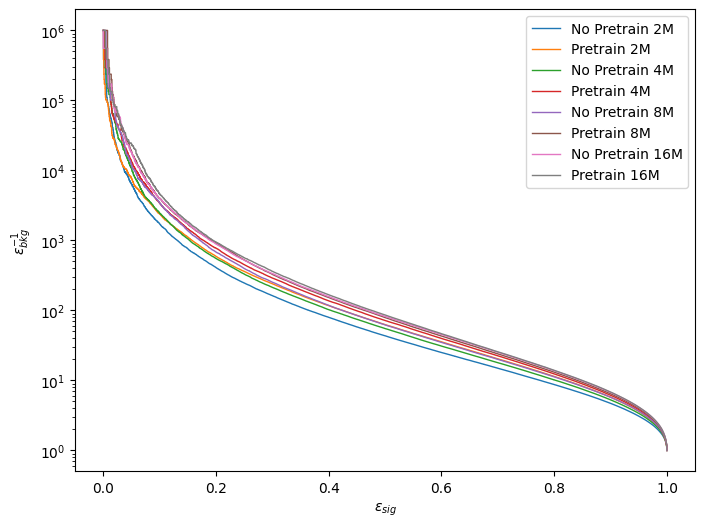
\includegraphics[width=0.75\linewidth]{figures/performance_curves.png}
    \caption{Background rejection $\varepsilon_{bkg}^{-1}$ plotted against signal efficiency $\varepsilon_{sig}$. Background rejection, or the inverse of the false positive rate, is used here because the ratio of signal to background in reality is very low so using background rejection makes it easier to visualize.}
    \label{fig:performance_curves}
\end{figure}

\begin{figure}
    \centering
    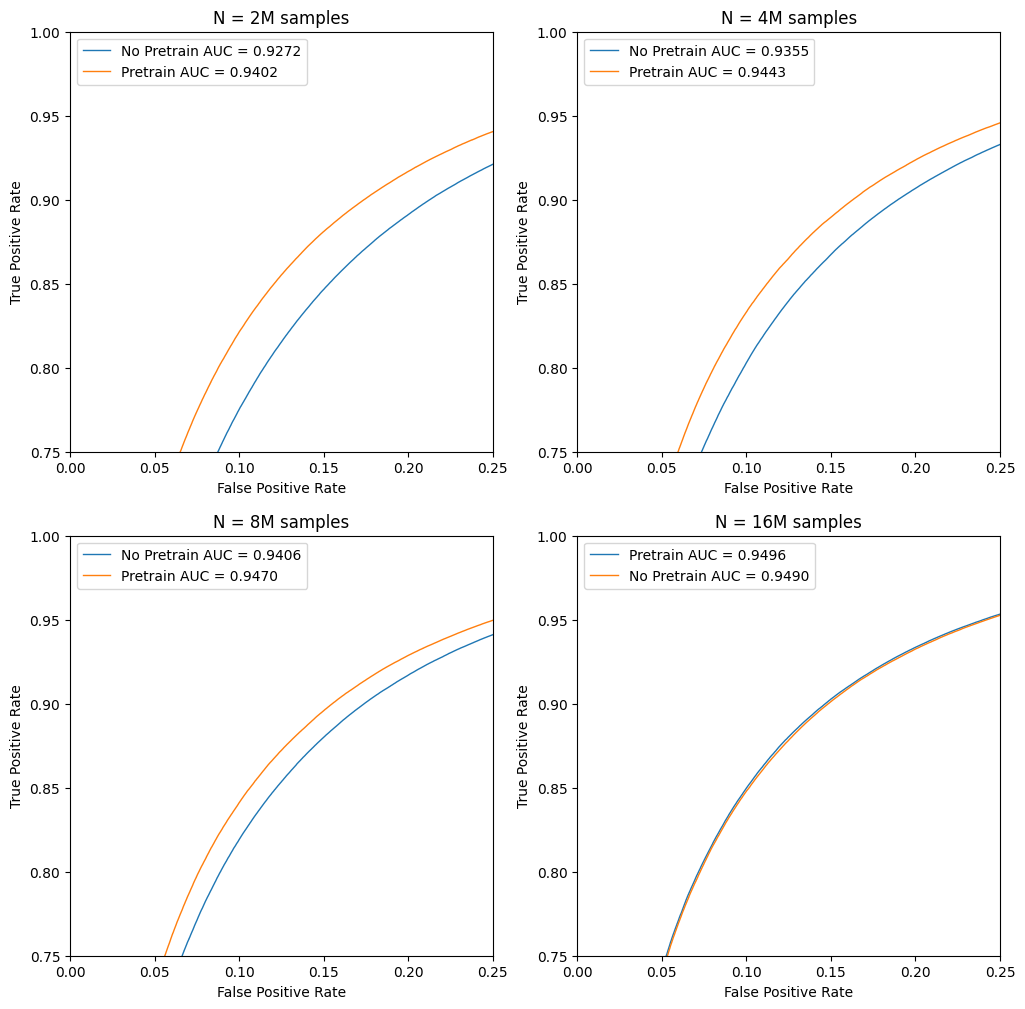
\includegraphics[width=1\linewidth]{figures/four_roc_curves.png}
    \caption{ROC curves plotted for pretrained and non-pretrained models trained on 2M, 4M, 8M, and 16M \textsc{Geant4} samples. Only one set seed is plotted.}
    \label{fig:four_roc_curves}
\end{figure}

\section{Training Speed}

Another advantage that using transfer learning has over training from scratch is a faster train time, as measured by number of training epochs required to find an optimal model. Figure \ref{fig:four_loss_curves} shows that pretrained models consistently converge to a better performing model in fewer epochs than starting from scratch. Numerical values for the optimal number of epochs are reported in Table \ref{tab:num_epochs}.

\begin{figure}
    \centering
    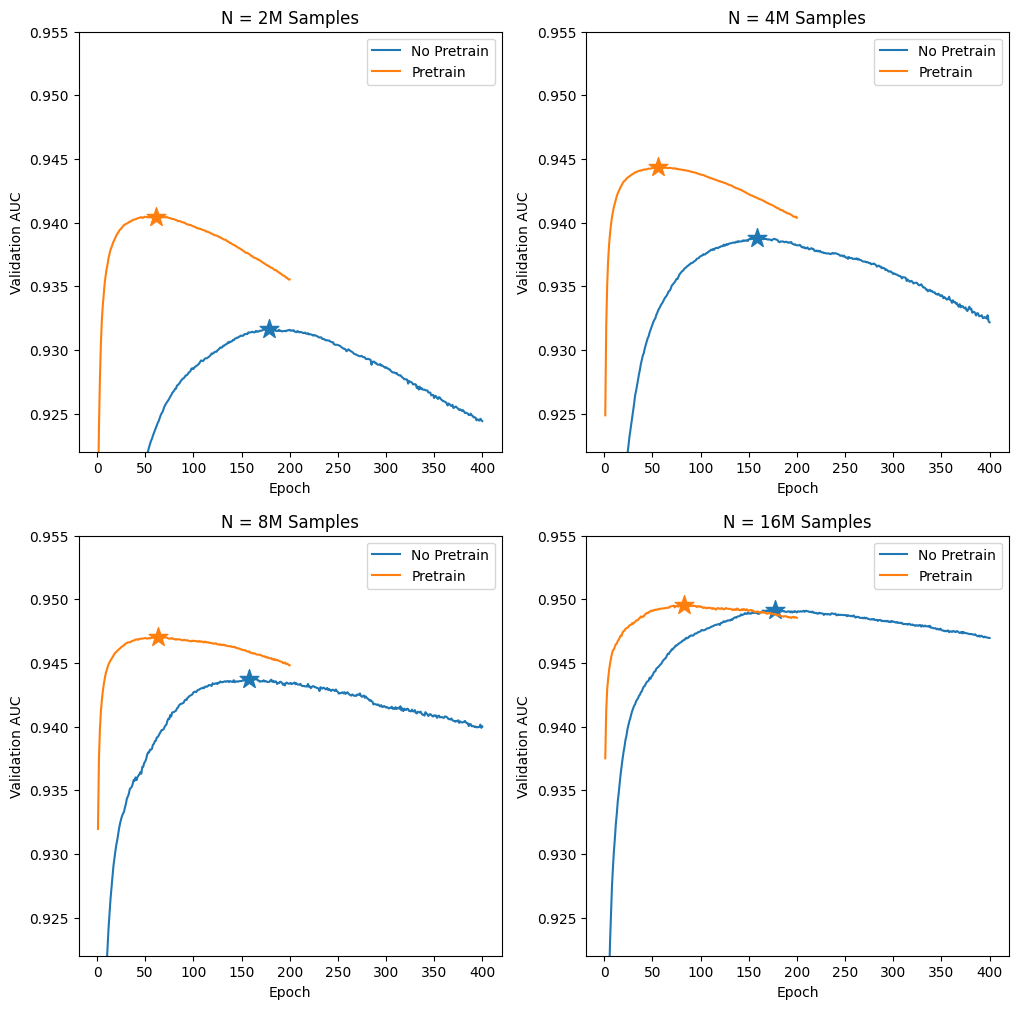
\includegraphics[width=1\linewidth]{figures/four_loss_curves.png}
    \caption{Validation ROC AUC scores plotted against training epoch. $N$ is the number of \textsc{Geant4} samples used in training. The epoch with the best AUC score is marked with a star. Only one set seed is plotted. Models with pretraining were stopped after 200 epochs due to decreasing performance.}
    \label{fig:four_loss_curves}
\end{figure}

\begin{table}[]
\centering
    \begin{tabular}{c|c|c}
    \hhline{===}
    \# Samples & No Pretrain & Pretrain \\ \hline
    2M  & 188.8 $\pm$ 12.5 & 55.2 $\pm$ 5.9 \\
    4M  & 155.0 $\pm$ 10.8 & 58.6 $\pm$ 4.8 \\
    8M  & 158.4 $\pm$ 29.0 & 66.6 $\pm$ 7.7 \\
    16M & 215.8 $\pm$ 25.7 & 86.0 $\pm$ 17.5 \\
    \hhline{===}
    \end{tabular}
    \caption{Number of epochs required before the best model was found. Model ranking is based on validation AUC. Reported values are the mean and standard deviations of five seeds. Lower is better.}
    \label{tab:num_epochs}
\end{table}
